\chapter{From corrective to predictive process control} \label{From Corrective to Predictive Process Control}
\minitoc

\section{Introduction}

This chapter describes an application of the previously proposed method to our industrial context. Since out-of-tolerance tank weight is the primary cause of part non-conformity, we investigate process parameters that contribute the most to the variability of tank weight. The first step is to gather a data set representative of the phenomenon to be modelled.  This historical data set is then used to model the relationship between process measurements and part quality. The results, as well as the difficulties encountered when applying such an approach in the industrial context studied will be discussed in detail. Finally, we will show how the results obtained in the framework of this research work have allowed us to identify some areas for improvement in our manufacturing process. 


\section{Motivation}

Poor quality or ``scrap'' parts are very expensive for a company like Plastic Omnium Clean Energy Systems. The “Cost of Non-Quality” (CNQ) is one of the key indicators most used by the company. However, when a part is declared bad, it is first necessary to understand the origin of the problem, which can require a lot of time and energy. Historically, Plastic Omnium industrial process monitoring has been driven using a knowledge-based corrective approach (Figure \ref{fig:Corrective process control}). The quality measurements of each product is used to adjust the process and to maintain the process capability. Moreover, some of the process parameters, which are considered as critic for process safety, are kept under control through the use of uni-variate control charts.  When a parameter falls outside the control limits, some warning messages are generated to alert the operators who have the task of regulating the machine so that the parameter can return in a safe zone. 

\begin{figure}
\centerline{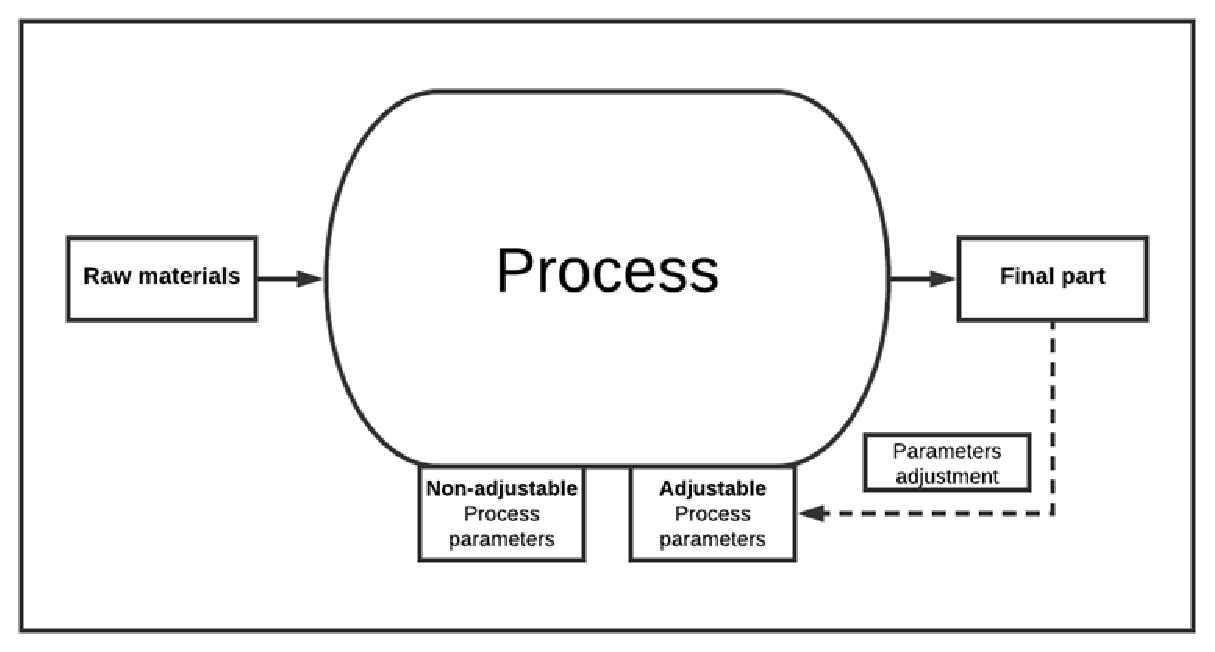
\includegraphics[scale=0.7]{images/chapter_3/corrective_approach.eps}}
\caption{Corrective process control}
\label{fig:Corrective process control}
\end{figure}

Evidence has shown that the overall stability of the process ensures, in most cases, the stability of the product quality. However, it still remains unclear how the system parameters impact the variability of product quality. Quality prediction would allow better adjustment of system parameters at an early stage of production. In other words, anticipation of product quality could be used to adjust the process in real time rather than retrospectively (Figure \ref{fig:Predictive process control}). Such an approach would allow process failures to be anticipated and corrected just-in-time, with an overall reduction in the production of non-conforming parts.

\begin{figure}
\centerline{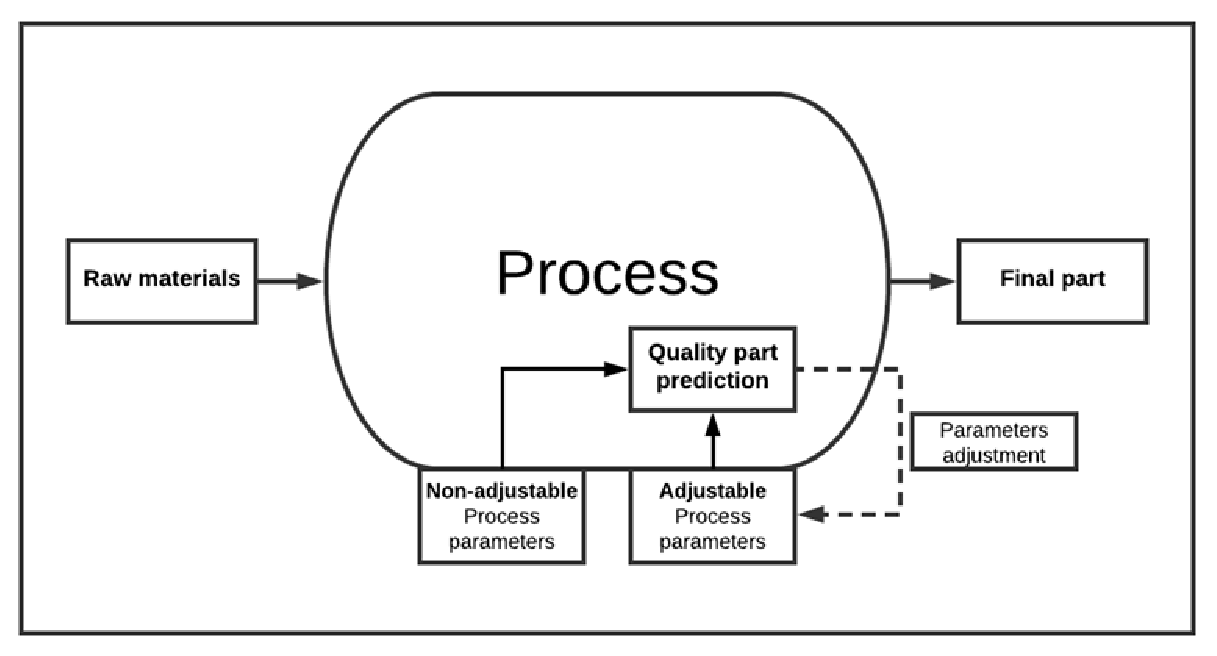
\includegraphics[scale=0.7]{images/chapter_3/predictive_approach.eps}}
\caption{Predictive process control}
\label{fig:Predictive process control}
\end{figure}

In order to understand the correlation between process parameters and the quality of the final part, we use a supervised learning approach. We view our complex industrial process as a black box with multiple inputs and one output. Given $p$ process parameters $(X_1,X_2,\ldots,X_p)$ and one product quality variable $Q$, we look for the function that better approximates the relationship between inputs and the output. Mathematically speaking, we look for the function $f$ that approximates the relationship between the process variables and the quality result:

\begin{equation}
    Y = \hat{f}(X_1,X_2,\ldots,X_p) + \epsilon
    \enspace,
\end{equation}
where $\epsilon$ is defined as the part of $Q$ that cannot be predicted from the input process parameters $(X_1,X_2,\ldots,X_p)$.

By an automatic analysis of a set of examples (training set) of measured input-output behaviour of the process, learning algorithms can find out important correlations between process variables and construct classifiers for detecting dangerous or unwanted process states.

In the context of our research framework, we have carried out a work in order to determinate what are the main causes of scraps involving the extrusion blow-moulding process. An analysis conducted on three years of data collected by the Manufacturing Execution System (MES) software of the company in a French plant has highlighted that the first cause of scraps in blow-moulding machines is due to tanks whose weight does not meet the customer's specifications. This kind of non-compliance accounts for about one half of the total amount of scraps (Figure \ref{fig:Most common scrap causes (2017-2018-2019)}) followed by inclusion and other contamination problems. 

\begin{figure}
\centerline{
\includegraphics[scale=0.9]{images/chapter_3/Scraps_codes.eps}}
\caption{Most common scrap causes (2017--2019)}
\label{fig:Most common scrap causes (2017-2018-2019)}
\end{figure}

% As presented in Section \ref{The key quality characteristics of a blow-moulded fuel tank}, the tank weight is historically considered as an important product characteristic as it provides an overall indication about the amount of material that composes the fuel tank. By ensuring a lower tolerance limit of the weight it is possible, according to experts, to ensure that there is enough material to ensure compliance of thicknesses. In the same way, there exist an upper tolerance limit which exists to ensure that the part it is not to heavy. By measuring in real-time, for each part produced, the weigh of the tank, people in plants feel reassured about the correct material distribution along its surface.  
As a consequence of this analysis, we decided to focus our efforts on trying to understand where these scraps come from and what we can do to try to reduce them. Moreover, since the weight is measured in real-time, it is possible to easily assemble a dataset composed of multiple samples. By following the approach described in Section \ref{Proposed Method} of this chapters, we aim to search for any hidden pattern or correlation within process data and quality data that could explain why some parts are not compliant in term of weight.


\section{Data collection}

\subsection{Process parameters of the SCADA software}

More than 5000 parameters are measured in real-time at each production cycle of our industrial process. Among these features, some are considered by the experts as critical to ensure the proper stability of the process (see Section \ref{The key parameters of the Extrusion Blow-moulding}). In addition to the critical process parameters there are timer and counter variables. A timer variable accounts for the time needed to execute a particular mechanical movement in the machine production cycle. The sum of all the mechanical times corresponds to the machine cycle time. A counter variable, instead, increases over time because of a particular event. For example, the number of parts produced in a production day is recorded in a counter variable.  

Process parameters are collected by the internally developed SCADA system and data are stored in multiple databases in accordance with the sources of each one. For instance, all the extrusion process data are stored in a database. The same is true for the blow-moulding data and for the weight of the tank that are stored in two separate databases. 

Each process parameter measured in real-time during the production process needs to be associated to the scalar value corresponding to the quality measurement of the manufactured product, at the end of the production cycle. In order to do that, the SCADA software computes some aggregate data to summarise the information in a limited set of scalar features. For each variable belonging to a production cycle, the average, maximum and minimum values are calculated. Then, the SCADA software attaches the aggregates data belonging to a production cycle to a specific traceability serial number which can be used as key to link the different sources of data. 

The extrusion blow-moulding process studied in this work has no system for measuring the parison length. As explained in Section \ref{Industrial domain: extrusion blow-moulding}, the parison length provides information about the material distribution.  Below we present the approach we have used to measure the parison length in real-time.

\subsection{Parison length estimation by computer vision}

The parison length is not available in our process data database because it is not measured. We looked for a measuring system having the following properties:
%
\begin{enumerate}
    \item relatively low software and hardware costs,
    \item requiring little expertise to adapt the model or process the data,
    \item adaptable to changes (for example, adaptable to any blow moulding machine in Plastic Omnium's plants),
    \item making analyses in real time, returning the result with low latency,
    \item able to operate in hostile environments,
    \item be robust to environmental variations (e.g. the system must operate day and night, regardless of lighting conditions).
\end{enumerate}
%
To meet these industrial constraints, we opted for computer vision. Our choice is motivated by the low cost of a camera, its ease of deployment, and the capabilities of deep learning-based models to detect objects in images. In Section \ref{Convolutional Neural Network} we shown how Convolutional Neural Networks reach state-of-the-art results in image classification, object detection and image segmentation tasks. We therefore chose this solution  to detect the parison to measure its length in real time.
The length measurement involves two main stages:
\begin{itemize}
    \item Parison detection: the parison should be detected inside the field of view of the camera. A CNN is trained to detect a (tight) bounding box containing the parison. 
    \item Length measurement: once the parison is detected, its length corresponds to the height of the bounding box.
\end{itemize}

The CNN architecture we chose is \textit{SSD MobileNet-V2}  (see Section \ref{Single Shot MultiBox Detector}), which presents an interesting trade-off between inference speed and model performances in the wild. Here, we expect 
In order to train such a model, 200 images of parisons were collected using a camera of HD resolution ($1280\times720$). By taking images of parisons during extrusion, we built a dataset representative of all possible parison lengths. All images were then annotated using the open source software \textit{Labelme} \citep{wada2016labelme} (Figure \ref{fig:input_and_label}). It is therefore possible to retrieve the bounding box containing the parison.   
\begin{figure}
\centerline{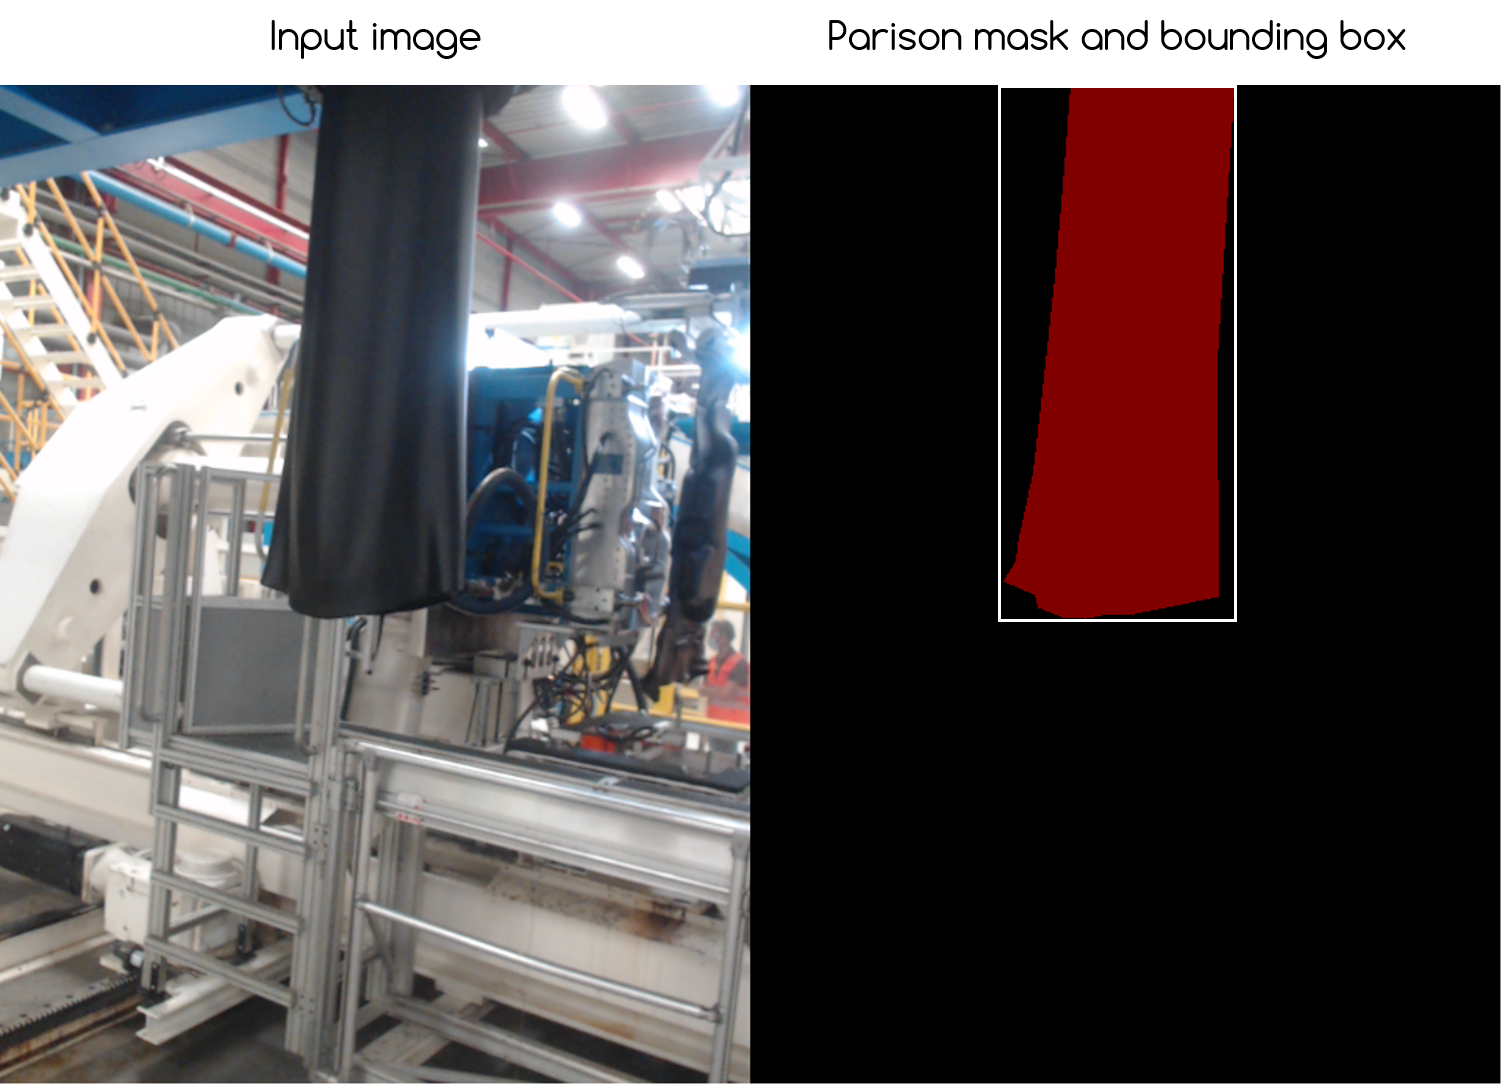
\includegraphics[scale=0.4]{images/chapter_3/input_and_label.png}}
\caption{Input image and parison mask}
\label{fig:input_and_label}
\end{figure}

The data was split into three different subsets: a training set (70\%), a validation set (10\%) and a test set (20\%). The training set samples are used to train the model, the validation set is used during the training to evaluate the performance of the model on unseen samples and to eventually stop the training if the model tends to over-fit. The test set constitutes the subset of samples used to evaluate the performance of the trained model on previously unseen data. The model was trained to minimise the loss function using the  \textit{Adam} optimiser~\citep{kingma2014adam} with the default parameter values ($\beta_{1} = 0.9$, $\beta_{2} = 0.98$ and $\epsilon = 10^{-9}$). The loss function used to train such as model is a combination of a \textit{Localisation loss} and a \textit{Confidence loss}. The localisation loss is the mismatch between the ground truth box and the predicted boundary box. The confidence loss is the loss of making a class prediction. For every positive match prediction, we penalise the loss according to the confidence score of the corresponding class.
% SHOULD I ADD MORE INFORMATION ABOUT THE LOSS ?

To limit the burden of data collection and annotation, we selected only  200 images and we used transfer learning (see Section \ref{Transfer Learning}), with the chosen architecture initialised with the pre-trained coefficients of the \textit{COCO} dataset \citep{lin2014microsoft}. The last linear layer of the model was replaced with a new one matching our problem. Since we are only interested in detecting parisons, the size of our last layer is one.  

SSD MobileNet-V2 provides accurate results in a limited amount of time. Figure \ref{fig:parison_inference} shows two ground truth boundary boxes from the test set and their corresponding prediction. The computation time is below $200$ millisecond on a \textit{Nvidia} Jetson Nano (a small computer equipped with a cheap GPU designed for embedded applications and deep learning based IoT). 
%
\begin{figure}
\centerline{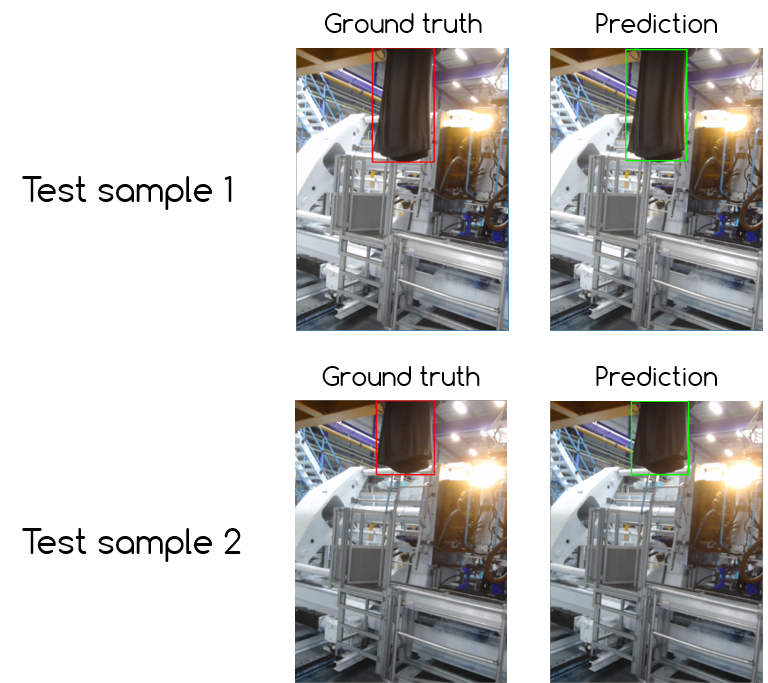
\includegraphics[scale=0.8]{images/chapter_3/parison_length_gt_prediction.png}}
\caption{Two parison length inference examples (from the test set)}
\label{fig:parison_inference}
\end{figure}
%
This system has proven to be robust and to meet the  industrial constraints identified, making accurate and reliable predictions in real time. A simple RGB camera and a small computer offer a cheap, non-intrusive solution that does not require any modification of the machine. 

With regard to our modelling approach we only care about the final parison. The parison length just before the mould closes to blow-mould the final part. We made the assumption that the final length could provide enough information to explain the weight variability.

% INTRODUCE THAT THE CAMERA CAN BE USED TO A BETTER PROCESS CONTROL   

Once the parison length acquisition was running online, we built a dataset with the SCADA software variables and the parison length measurement. We collected data from 5 different batches, corresponding to as many production days, for a total of 5597 samples and more than 5000 features. 

\section{Data processing}

Using all available variables, the number of input features is too large compared to the number of examples in the dataset. We applied two different procedures for variable selection: an expert-based procedure and a statistical-based procedure.

\paragraph{Expertise-based data procedure}

We relied on expert knowledge of the process to discard all features that are not relevant to explain the weight variability. For instance, all counter variables collected by the SCADA software do not bring any interesting information and can be removed. Also, many timer variables, representing the time needed to execute a particular mechanical operation, are redundant and provide no added value. Therefore, most of timer variables have been removed from the dataset.

\paragraph{Statistical-based procedure}

In order to further reduce the number of features, three different statistical feature selection approaches have been used, based on:
\begin{itemize}
    \item correlation between features , 
    \item feature variance,
    \item \textit{stability selection} (see Section \ref{Stability Selection}).
\end{itemize}
%
Removing highly correlated variables eliminates redundant features and reduces collinearity between features that can cause stability problems when fitting the regression model.
%When two or more predictor variables in the same regression model are correlated, they cannot independently predict the value of the dependent variable. In other words, they explain some of the same variance in the dependent variable, which in turn reduces their statistical significance. 
For each pair of features with a correlation value greater than 0.90, one of the two features was removed. Features with very low variance (constant or with no more than 3 different values) were removed. To further reduce the number of features, we applied stability selection. By generating bootstrap samples of the data, and by leveraging the ability of the LASSO penalty to estimate which features are important in each sampled version of the data, we are able to select only those features that have been selected for many perturbed versions of the original problem. Data were finally normalised to have zero-mean and unit-variance (see Section \ref{Data Scaling}). Normalising features is not only important if we are comparing measurements that have different units, but it is also a general requirement for many machine learning algorithms. Figure \ref{fig:data_processing} resumes the data processing flow.
%
\begin{figure}
\centerline{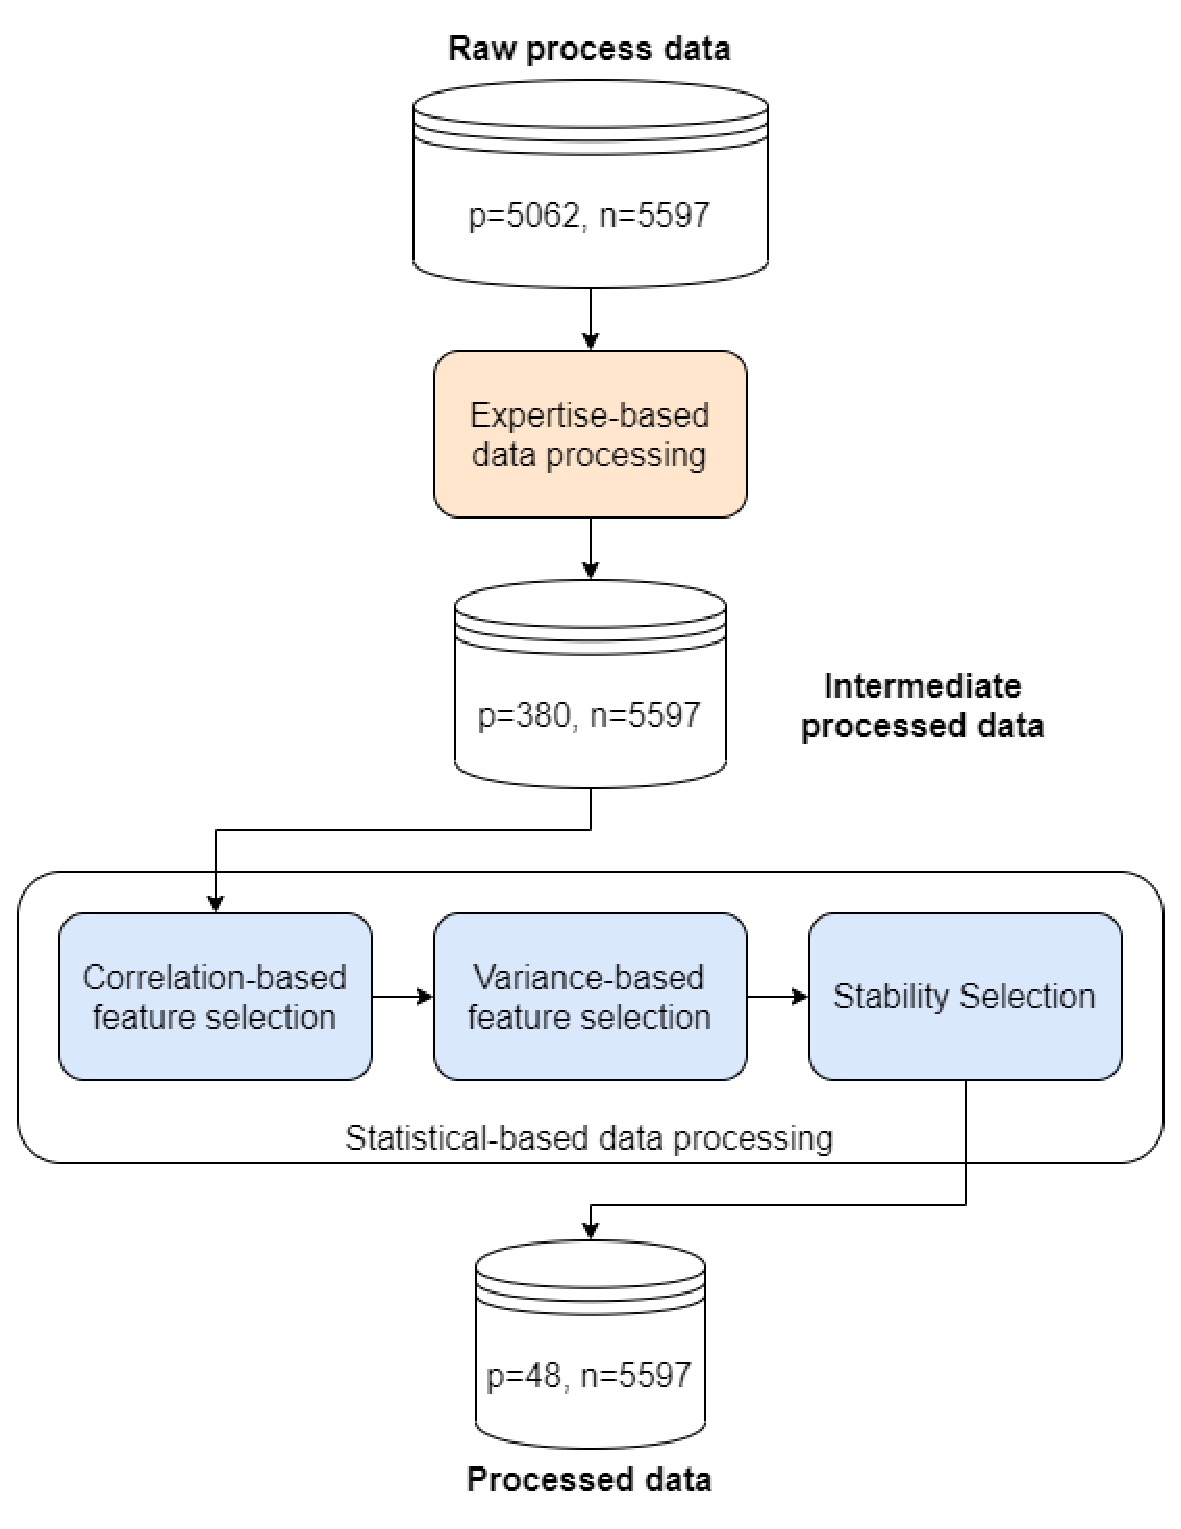
\includegraphics[scale=0.7]{images/chapter_3/Data_processing.eps}}
\caption{Data processing flow}
\label{fig:data_processing}
\end{figure}
%

\section{Exploratory data analysis}

\subsection{Weight versus parison length}

This was the first time that data on parison length was available. The relationship between the parison length just before the blowing phase and the weight of the blown part is illustrated by a scatter plot in Figure \ref{fig:length_weight_scatter}.
%
\begin{figure}
\centerline{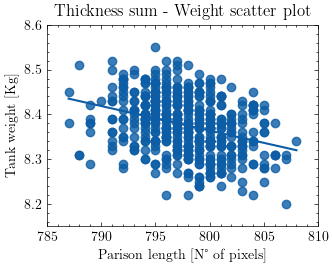
\includegraphics[scale=1.2]{images/chapter_3/length_weight_scatter.png}}
\caption{Parison length - Weight scatter plot}
\label{fig:length_weight_scatter}
\end{figure}
%
The plot shows a weak  negative correlation between the parison length and the weight. The Pearson correlation is equal to $-0.32$. The physical explanation is simple: the longer the parison, the less material remains inside the the mould during the blow-moulding. Moreover, the upper part of the parison is often thicker to prevent the parison from breaking under its own weight.  

\subsection{Low dimensional representation} \label{Principal Component Analysis for data exploration}

The large number of features makes it difficult to detect possible hidden patterns in our data by a direct visual representation. We use Principal Component Analysis (see Section \ref{Principal Component Analysis}) to produce the low-dimensional representation that best preserves the distance between examples. 
%
\begin{figure}
\centerline{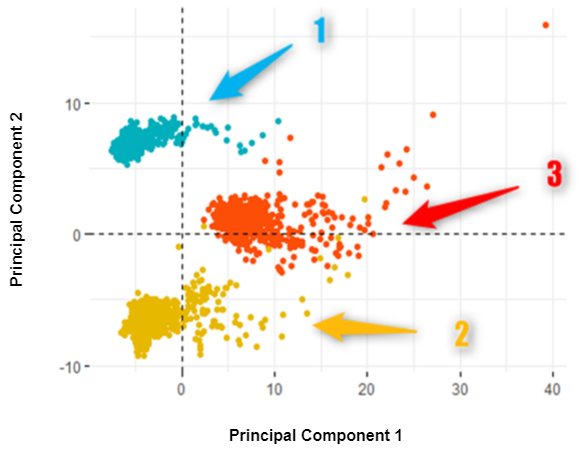
\includegraphics[scale=0.5]{images/chapter_3/PCA.png}}
\caption{Sample projection on the two first axes of Principal Components Analysis}
\label{fig:pca}
\end{figure}
%
Figure \ref{fig:pca} represents the projection of the samples from 3 batches on the first 2 principal components of PCA. This representation shows two major patterns:
\begin{itemize}
    \item Data are organised in clusters,
    \item For each cluster of data there exist a subset of points moving apart from the cluster.
\end{itemize}
%
Each cluster corresponds to a specific production day or batch. This means that, for the same tank reference, the process parameters differ more between each batch than within a batch. We will call this phenomenon the ``batch effect''. Moreover, the samples are at the periphery of the centre of each cluster correspond to tanks produced in the first two hours after the machine was started. This allows to identify two operating regimes: the \textit{transient} and the \textit{stable} regimes. During the transient regime, the process parameters are slightly different, particularly in terms of temperature. During the transient regime the rate of non-conformity rate in terms of weight is considerably higher (about 300\%) compared to the stable regime.    

\section{Supervised learning modelling}

Given our input processed data $P$ composed of $p$ process parameters and $n$ samples and the output vector $W \in \mathds{R}^{n}$ of the tank the role of the supervised learning modelling is to find the function $\hat{g}$ such that:
%
\begin{equation}
    \hat{g} = \argmin_{g \in \mathcal{G}} \sum_{i=1}^n (W_{i} - g(P_{i}))^{2} \enspace.
\end{equation}
%
We compared several models: ordinary linear regression, Lasso regression, ridge regression (see Section \ref{Parametric models}), random forest and gradient boosting tree (see Section \ref{Tree-based methods}). The choice of these algorithms is motivated by:
%
\begin{itemize}
    \item \textit{Interpretability}: Since we aim to understand which parameters most affect the weight of the blow-moulded tank, we are interested in applying interpretable models. Linear models and tree-based methods are considered to be among the most easily interepretable models.
    \item \textit{Performance}: These methods work quite well with tabular data. When dealing with tabular data, deep learning hardly surpass traditional machine learning algorithms \citep{shwartz2021tabular}. 
\end{itemize}
%
In order to evaluate the predictive power of our models, we used two different approaches: cross-validation and batch cross-validation. 

\paragraph{Cross-validation}

In standard cross-validation, called \textit{K-fold} Cross-validation, the training set is split into $k$ smaller sets. The following procedure is followed for each of the $k$ “folds”:
%
\begin{itemize}
    \item the model is trained using the remaining $k - 1$ folds as the training set,
    \item the error of the resulting model is estimated on the fold set apart from the training set.
\end{itemize}
%
The cross-validation criterion is then the average of error values computed in the loop.
%
\begin{equation}
    CV_{K} = \frac{1}{K}\sum_{i=1}^{K}score_{i}
    \enspace.
\end{equation}
%
This approach is computationally expensive, but does not waste too much data (as is the case when fixing an arbitrary validation set), which is a major advantage in problems where the number of samples is small. In our experiments we used five folds.

\paragraph{Batch cross-validation}

Instead of performing the cross-validation on $k$ random splits of the training set, we split the whole dataset according to the different batches (production days) to cross-validate the model on each batch. Since our dataset comprises 5 different batches, at each time, one batch is used as a validation set and the remaining 4 batches are used to fit the model.

\begin{equation}
    CV_{batch} = \frac{1}{n\degree\;batches}\sum_{i=1}^{n\degree\;batches}score_{i}
    \enspace.
\end{equation}

The mean of the 5 different scores is calculated to have an accurate estimate of the model prediction performance. With this strategy we evaluate whether the models are able to predict on an unseen batch.  


\section{Results and discussion} \label{Results and Discussions}

We use the $R^2$ metric to evaluate the models. Both cross-validation and batch cross-validation return negative $R^2$ values for all the models. 
This means that the models are worse at predicting the weight than the sample mean, and thus that the variability of the weight cannot be explained by the available parameters of the process. Results for cross-validation are resumed in Table \ref{tab:cross_validation_results}.  

\begin{table}[]
\centering
\caption{Cross-Validation results}
\label{tab:cross_validation_results}
\begin{tabular}{lllll}
\toprule
\textbf{Algorithm} & \textbf{R² train} & \textbf{R² test} \\
\midrule
Linear regression   & 0.72   & -0.34    \\ 
Lasso regression    & 0.80   & -0.25    \\ 
Ridge regression    & 0.78   & -0.26    \\ 
Random forest       & 0.94   & 0.05     \\ 
Gradient boosting   & 0.95   & -0.11    \\ 
\bottomrule
\end{tabular}
\end{table}


\begin{table}[]
\centering
\caption{Batch cross-validation results}
\label{tab:batch_cross_validation_results}
\begin{tabular}{lllll}
\toprule
\textbf{Algorithm} & \textbf{R² train} & \textbf{R² test} \\
\midrule
Linear regression    & 0.50   & -1.34  \\ 
Lasso regression     & 0.62   & -0.45  \\ 
Ridge regression     & 0.67   & -0.39  \\ 
Random forest        & 0.81   & -0.27  \\ 
Gradient boosting    & 0.76   & -0.73  \\ 
\bottomrule
\end{tabular}
\end{table}

Both tables highlight how all the approaches tend to over-fit but struggle in generalise what has been learned on the train set to unseen new samples. This is especially true for tree-based methods that in general are more prone to over-fit. 

Results are quite astonishing but are showing evidence that it could be hard to apply statistical models in a field, manufacturing industry, where there is a lot of uncertainty. A further analysis was conducted to try to explain and motivate these results. We have identified six possibles reasons for these negative results:
%
\begin{enumerate}
    \item \textit{Non-stationarity of data}
    \item \textit{Lack of data characterising the properties of the raw material}
    \item \textit{Low variability in product quality}
    \item \textit{Reliability of the input data}
    \item \textit{Weight too resultant}
\end{enumerate}
%
The following paragraphs provide more detail about each  source of error identified. 

\paragraph{Non-stationarity of data}

Results obtained with batch cross-validation show that our models do not generalise among different batches. Actually if we look at distributions of our input features we can see how they change considerably among different batches (Figure \ref{fig:Example of a process parameter variability in probability distribution}). 
%
\begin{figure}
\centerline{\includegraphics[scale=0.4]{images/chapter_3/process_parameter.eps}}
\caption{Probability distributions across batches for a particular process parameter}
\label{fig:Example of a process parameter variability in probability distribution}
\end{figure}
%
A “Two-sample Kolmogorov-Smirnov” test was applied to all pairs of batches. According to these tests, only 35\% of the input features share the same probability distribution over all batches (at a $0.95$ confidence level).
Standard machine learning models rely on stationarity hypothesis to generalise: a trained model expects that the test distribution follows the distribution of data used to train the model.

\paragraph{Lack of data characterising raw material properties}

The change in data distribution may also be due to some external events or factors that we do not control and do not take into account within our own input process data. We claim that the ``batch effect'' we observe in the data could be a consequence of certain changes in the rheological properties of raw materials. In fact, the final part is the result of the transformation of raw material through our complex process. Unfortunately, to this date, these data are not available and they cannot be integrated in our dataset. Further studies have been carried out in order to see if it is possible to measure some rheological properties of the material in real-time. There are industrial on-line rheological systems that provide continuous measurements of the melt flow rate or apparent viscosity directly on the manufacturing process. Unfortunately, this solution is not economically viable, especially as such a system would have to be installed for each of the 6 screws.

\paragraph{Low variability in product quality}

The manufacturing process is already relatively reliable and stable, with low variability in product quality. The scrap rate is under 3\% and the tolerance limits set to evaluate the compliance of blow-moulded tanks are quite strict. In general, a weight variability of about 300 grams is sought, which for an average tank weight of $8.5$ kilograms corresponds to about $3.5\%$ of the total weight. The phenomenon modelled would have been more pronounced, and the problem would have been simpler with a larger weight variation.     

\paragraph{Reliability of the input data}

As we look for small variations of weight, it is important that the input data is accurate enough. In an industrial environment, such as a production plant, the collected data are most of the time noisy. The maintenance of the sensors cannot be done regularly. As a consequence, some sensors may provide erroneous values. Moreover, the SCADA software computes some aggregate operation on the input time series-data, which can lead to a loss of information. Finally, it is quite complex to attach extrusion data to the traceability serial number of a tank since extrusion is a continuous process and there are no precise triggers to define what data belongs to a given part. The extrusion data may be misaligned with the manufactured part.  

\paragraph{Weight too resultant}

Another possible explanation is directly related to the nature of the output variable considered in our problem, the weight. In fact, the weight is a resulting variable which depends on the distribution of the material on the tank surface. However, different material distributions can produce the same final weight. In others words, different manufacturing conditions, represented by different process parameters values can lead to the same weight. As a consequence, the model struggles to learn the function which approximates the relationship between process parameters and quality data.

These results highlights the difficulties we can encounter when dealing with manufacturing process data. However, in the following section we will show how the work presented in this chapter has made it possible to start a new project to improve the manufacturing process. 


\section{SmartBMM: towards smarter machines}

The data analysis results presented all along this chapter have shown the inability to explain the tank weight variability given the blow-moulding process data that are considered as critical by process experts. The possible reasons have been discussed in detail in the previous section. What the analysis has also highlighted is that the most scrap occurs just after the machine start-ups (see Section \ref{Principal Component Analysis for data exploration}). As shown previously, right after the machine start-up, the extrusion blow-moulding process is not completely stable which increases the overall scrap rate of the blow-moulded parts. Moreover, an interview of different extrusion blow-moulding experts has highlighted that there are no common and shared best practices to start the machine. As a consequence,  there is a lot of variability between startups.

\begin{figure}
\centerline{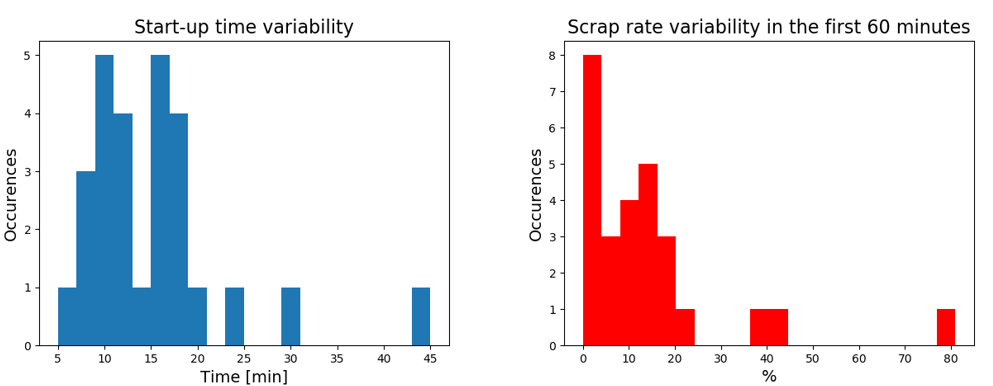
\includegraphics[scale=0.7]{images/chapter_3/smartbmm_barchart.png}}
\caption{Time and scrap rate variability for 27 machine start-ups in a Plastic Omnium plant}
\label{fig:smartbmm_barchart}
\end{figure}
%
Figure \ref{fig:smartbmm_barchart} illustrates this variability among 27 machine start-ups performed in a Plastic Omnium plant. On the left bar-chart, we can see how the time needed to start the machine changes from a start-up to another. Sometimes the start-up is done in 10 minutes, other times a full one may take around 15-20 minutes. There are also three occurrences for which the start-up took more than 20 minutes. The right bar-chart reports the scrap rate in the first 60 minutes. Most of the time, the scrap rate does not exceed 5\%, but there are some starting for which the scrap rate is above 10\%. These observations call for some efforts to improve the way the extrusion of blow-moulded machines is started. By automating and by optimising the machine start-up we should reduce the uncertainty introduced by manual starts. This would allow for a faster convergence towards the stable regime of the machine and, as a consequence, to a smaller number of part non-conformities.   

%We are aware that the scraps may have a multitude of reasons which do not depend on the way the machine is started, but we claim that providing repeatable and optimised starting should benefit at the overall performance of the manufacturing process. 
The project was initially conceived to handle just the machine starting phase but later on, it was extended to also cover the purge cycles of the machine. Indeed, ensuring good purge cycles reduces the risk of contamination/inclusion problems. In this context, we have developed the \textit{SmartBMM} solution. \textit{SmartBMM} is a software which leverages the real-time data collected directly from the PLC of the machine and the past data to follow the best instructions to get the machine started without any manual intervention of the operators.

\begin{figure}
\centerline{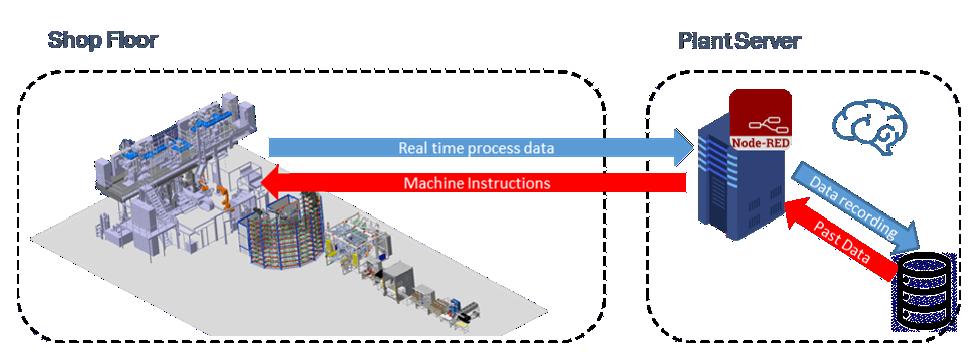
\includegraphics[scale=1]{images/chapter_3/SmartBMM.eps}}
\caption{\textit{SmartBMM} software}
\label{fig:SmartBMM}
\end{figure}

Figure \ref{fig:SmartBMM} shows broadly how the SmartBMM works. The SmartBMM software collects real time data directly from the PLC and stores it in a database for later retrieval. When the SmartBMM software is started the data collection continues, but, this time, the machine starts to write information to the PLC to execute a set of operations. The software takes the real time incoming data and the past data to elaborate the machine instructions to bring the machine to production conditions. The stored data are used to compute production extruder speeds which, accordingly to past data, minimise the non-conformity rate. Looking at previous production runs we are able to retrieve the process conditions which lead to a better performance and a lower scrap rate. The software is developed using the \textit{Node-RED} \citep{nodered} programming tool. Node-red is a low-code programming for event-driven applications which was specifically designed to work with IoT and that allows easy interfacing with machines through different communication protocols.

Instead of manually start the machine by pressing simultaneously multiple buttons on the HMI (Human Machine Interface), machine setters and operators have to press only one button to start a cycle, whether it is a \textit{starting} cycle or a \textit{purge} cycle.  

\begin{itemize}
    \item The starting functionalities leverages the real-time data collected directly from the PLC of the machine and the past data to elaborate the best instructions to get the machine started without any manual intervention of machine operators. The set of consecutive instructions provided to the machine are fairly standard. The extruders are started, then the material is fed into the screw, then the extruder speed is raised and so on. However, our system does not rely on timers to trigger the machine instructions. In real time the process status is controlled and the next machine instruction is triggered only if the process meets all requirements.
    Two starting functionalities are available: \textit{full} and \textit{downtime}. The first one executes a starting phase when the machine is completely stopped; the second one returns to the production condition in which the machine was temporarily idled.
    %  There exist two Purge cycles: the \textit{Purge Out} and the \textit{Purge In}. The Purge Out cycle is done when the machine is stopped for more than 2 hours to remove any FINIRE. The Purge In is done every time that the Purge Out has been done to prepare the extruder for the production run. 
    \item The purge functionalities allow to improve purge cycles of the machine.
    During purge cycles we want to ensure that enough material transits into the extruders at high pressure to clean them of residual production material. Instead of relying on fixed speed values or timers, we have developed a \textit{PID controller} that regulates the extruder speeds to ensure that they are constantly above the pressure targets. Moreover, the amount of material transiting through the screws is controlled in real-time. This allows to finish the purge cycle only when the correct amount of material has transited through the screws.     
\end{itemize}
%
The starting and purge functionalities reduce the ``weight not OK'' and the ``contamination'' scraps, which account for $2/3$ of the total amount of non-conformities.
The functionality is chosen by the operator through a graphical user interface (GUI) specifically developed to allow an easy interaction with the software (Figure \ref{fig:SmartBMM_gui}).
%
\begin{figure}
\centerline{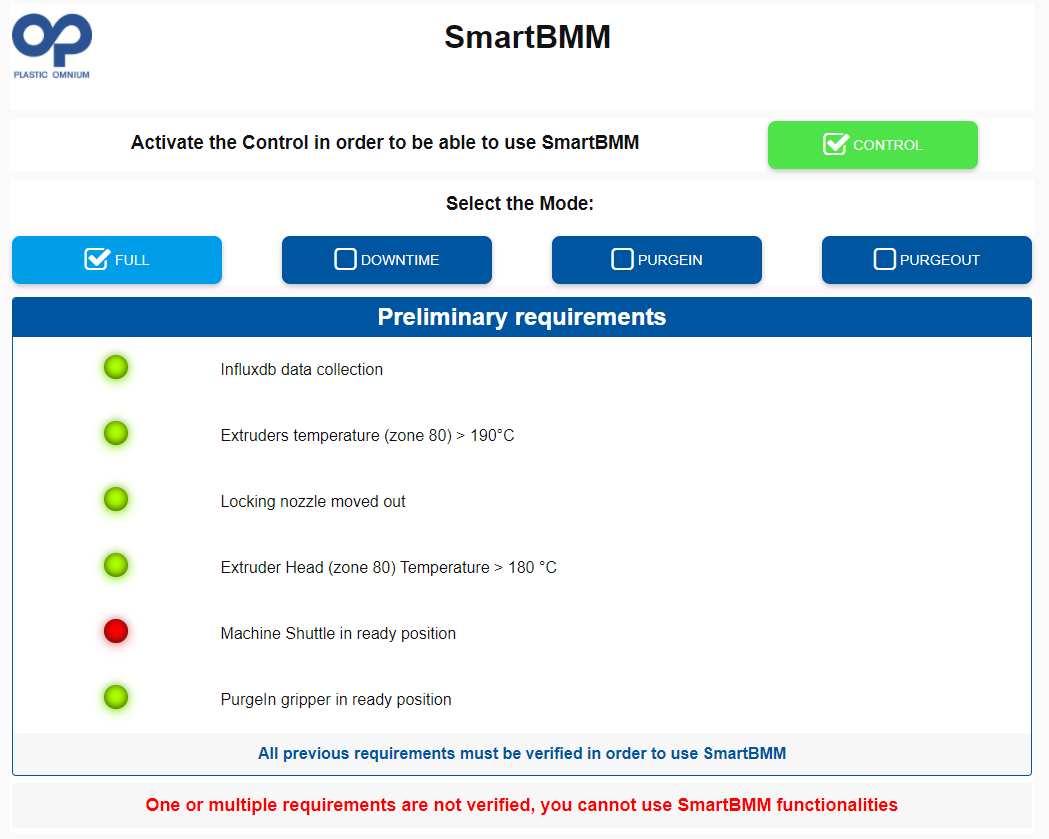
\includegraphics[scale=0.5]{images/chapter_3/SmartBMM_gui.png}}
\caption{\textit{SmartBMM} GUI}
\label{fig:SmartBMM_gui}
\end{figure}
%
Historically, all manufacturing processes, including extrusion  blow-moulding, rely on PLC programs to execute the set of instructions to allow the manufacturing machine to work correctly and to allow for the transformation of raw materials into finished products. In this project, we decided to pilot the machine outside of the machine PLC for the following reasons:
%
\begin{itemize}
    \item PLCs are very robust and safe, but they lack flexibility. PLCs are conceived to execute a set of logical instructions but they do not lend themselves well to be used concurrently with other systems such as databases. Developing a more complex logic which involves data storage and communication with databases is by far more easy with traditional software development tools.
    \item Implementing the logic on an external system such as a physical or a virtual server reduces the number of PLC modifications of the machine. Our software is  non-intrusive and can be installed remotely on a server without any direct modification of the PLC program. It is something that can be plugged to the machine to introduce new functionalities. This reduces costs considerably, since it does not require the intervention of an external consultant.
\end{itemize}
%
This strategy has, however, a main drawback. Our tools completely rely on plant network to communicate instructions to the PLC. Which means that a bad network could be a bottleneck for the correct functioning of our software. Security features have been added on the software side to interrupt the communication with the machine if any network failures prevents to communicate with the machine.
In our opinion this is an example of a cyber-physical system. SmartBMM leverages the sensor networks with data processing to monitor and control physical environment, with feedback loops able to elaborate the best set of machine instructions given the different process conditions.


\section{Conclusion}

In this chapter, we have presented an empirical evaluation of our approach in the industrial context. The features currently collected by home made \textit{SCADA system}, even when enriched by parison length measurements, cannot predict the tank weights. These results show the difficulty of applying statistical models in batch manufacturing industries, where it is not always possible to have knowledge of all the elements that contribute to the variability of the part quality. Possible explanations for these results were discussed. Nevertheless, this research work has allowed the identification of avenues for improvement of the blow-moulding process. In particular, the exploratory data analysis has shown how most of the part non-conformities occur just after machine start-up, when the process is not yet stable. This led to the launch the \textit{SmartBMM} project.

\subsection{Scientific Contribution}

The results presented in this chapter question the effectiveness of data-driven methods in certain manufacturing contexts. The end-to-end data-driven methods have proven to be effective in many applications, but for them to work well, informative data on a stationary phenomenon is required. In other situations, it may be better to decompose the original problem into several sub-problems with properly controlled data quality. The following chapter will present such an approach.

\subsection{Industrial Contribution}

This chapter presents three main industrial contributions.
\begin{itemize}
    \item Firstly, the work challenges certain beliefs about the operation of the blow-moulding process. The process parameters considered critical to ensure proper functioning of the process do not explain the variability in tank weights. The control limits previously set for the critical parameters of the process to ensure the correct functioning of the production process were found to be insufficient for providing such an explanation.
    \item The parison length measurement has opened new research perspectives. By measuring in real-time the length of the parison, we will eventually be able to control the distribution of material over the entire length of the parison to improve the quality of the manufactured parts. Further information and perspectives will be presented in Chapter \ref{Contributions and perspectives}.
    \item Finally, the \textit{SmartBMM} software that was developed starting from the results obtained trough the data analysis process has been used to improve the machine start-up phases which lead to a high scrap rate. By ensuring a better start-up, we reduce the transient phase and thus the percentage of parts that do not meet quality standards. Future works will make use of the parison length measured by the camera to add to SmartBMM new functionalities.  
\end{itemize}

